\documentclass[twoside,11pt]{homework}
\usepackage{bbm}
\usepackage{graphicx}

\coursename{MECS4510 Evolutionary Computation, Fall 2023} 

\studname{Bole (James) Pan}    % YOUR NAME GOES HERE
\studmail{bp2632@columbia.edu}% YOUR UNI GOES HERE
\hwNo{1}                   % THE HOMEWORK NUMBER GOES HERE
\date{September 17, 2023} % DATE GOES HERE

% Uncomment the next line if you want to use \includegraphics.
%\usepackage{graphicx}

\begin{document}
\maketitle
\begin{itemize}
    \item UNI: bp2632
    \item Instructor: Prof. Hod Lipson
    \item Grace hours used: 0 
    \item Grace hours remaining: 96
\end{itemize}
\newpage


\section*{Performance Plot}

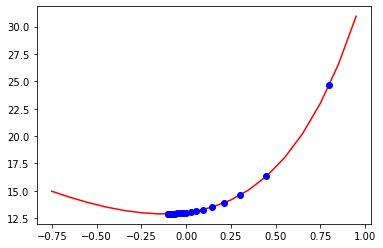
\includegraphics[width=0.9\textwidth]{output.png}

\section*{Methods}
\begin{itemize}
    \item \textbf{Representation Used:} We represent each city as a tuple with two elements. 
    A route (individual) is an ordered array of all the cities. A population is an array of routes (individuals).
    We are using direct representation, and more specifically, index representation.
    \begin{itemize}
        \item \textbf{Mutation}: We use the swap mutation method. For an individual route, we loop through each city, and with a certain mutation rate
        we probablistically swap this city with another random city. 
        \item \textbf{Crossover}: We use the order crossover method. For two parent routes, we randomly select a subset of cities from one parent, and make the child's corresponding segment the same as that parents'.
        then fill in the rest of the cities in the order of the other parent.
    \end{itemize}
    \item \textbf{Random Search}: Randomly generate a permutation of the cities and calculate the total distance. Repeat this process for a number of times and record the best result.
    \item \textbf{Random Mutation Hill Climbing}: Randomly generate a permutation of the cities and calculate the total distance. Then, for a number of times, apply mutation on the route and calculate the fitness of that route. 
    If the new fitness is higher, keep the new route. Repeat this process for a number of times and record the best result.
    \item \textbf{EA variation and selection methods used}: We use the roulette selection method. From the initial population, we first select a small population of elites. The higher the fitness, the more likely an individual would
    be selected for this group. We put all our elites in the new population. Then, until the new population reaches the predetermined populationwe size, we randomly select two individuals from the elites and apply crossover to produce a child,
    apply mutation on the child, and put it into the new population. This process, going from the initia population to the new population, is repeated for a number of times (called generations).
    \item \textbf{Analysis of Performance}:
    \item \textbf{Methods compared}: we compare the performance of random search, random mutation hill climbing, and EA.
\end {itemize}

\end{document} 
